\documentclass{article}
\usepackage{geometry}
\usepackage{float}
\usepackage[T1]{fontenc}
\usepackage[polish]{babel}
\usepackage[utf8]{inputenc}
\usepackage{graphicx}
\graphicspath{ {./images/} }

\geometry{
 a4paper,
 total={170mm,257mm},
 left=20mm,
 top=20mm,
}

\title{Analiza i przetwarzanie dźwięku - Projekt 3}
\date{\today}
\author{Mateusz Śliwakowski}

\begin{document}
  \pagenumbering{gobble}
  \maketitle
  \pagenumbering{arabic}
  
\section{Treść zadania}
Celem zadania było zaimplementowanie programu, który wczytuje plik audio a następnie przeprowadza jego analizę w dziedzinie częstotliwości na poziomie ramki. Należało zbadać cztery parametry - \textit{Volume, Frequency Centroid, Effective Bandwidth} oraz \textit{Band Energy}.

\section{Opis aplikacji}

Aplikację zdecydowałem się wykonać w języku \textit{C\#} w środowisku \textit{WinForms}. Jako, że w zadaniu można było wykorzystać znaczną część implementacji z projektu 2 zdecydowałem, że zamiast tworzyć nowe rozwiązanie, projekt zrealizuję poprzez rozwój poprzedniego. Prace rozpocząłęm od dodania zakładek z nowymi parametrami.

\begin{figure}[H]
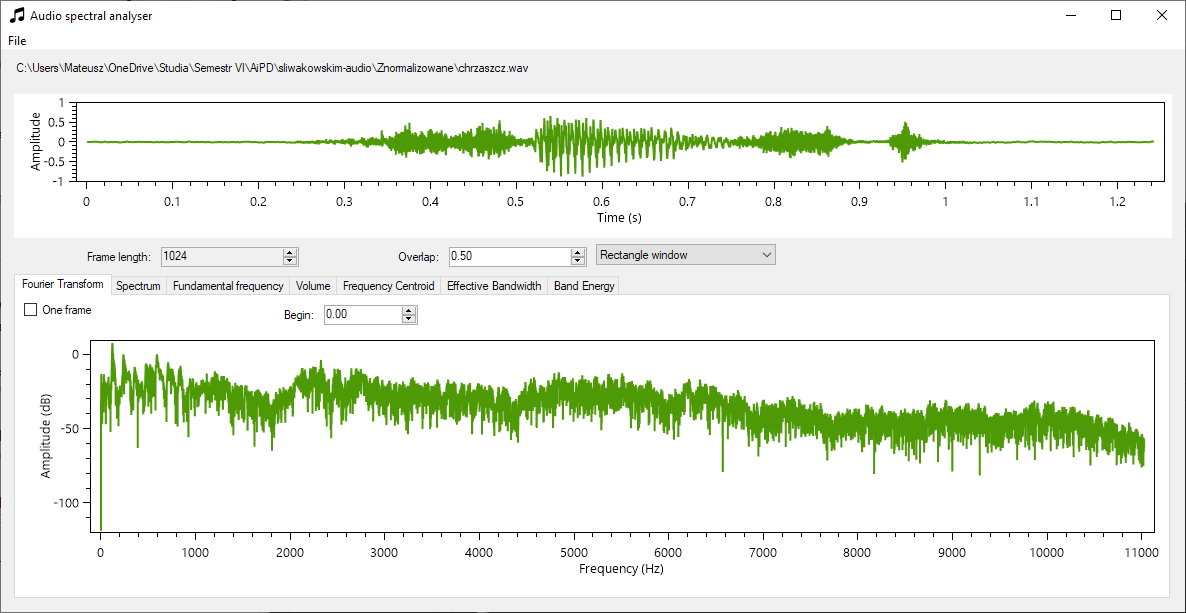
\includegraphics[width=6in]{scr1.png}
\centering
\caption{Interfejs użytkownika}
\label{fig:interface}
\end{figure}

\section{Zaimplementowane metody}

\section{Wyniki działania programu}

\section{Wnioski}
\subsection{Implementacja}

\subsection{Wyniki analizy audio}


\begin{figure}[b]
\centering
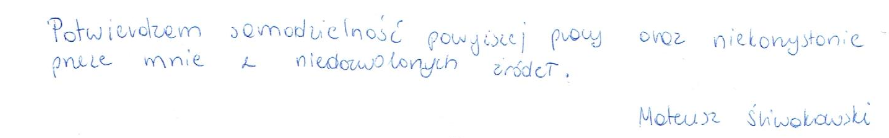
\includegraphics[width=5in]{bottom.png}
\end{figure}

\end{document}

